\chapter{Introduction}

\section{Statistiques et probabilité}
\
Les statistiques consistent à l'analyse de données issues de phenomènes aléatoires. 
Elles servent à comprendre la \textbf{variabilité des données} et à permettre des \textbf{prédictions} sur des phénomènes futurs.

\begin{exemple}
    Voici quelques exemples de situations où les statistiques sont utilisées :
    \begin{itemize}
        \item La météo : les prévisions météorologiques sont basées sur l'analyse de données.
        \item Résultats d'une élection : les sondages sont utilisés pour prédire les résultats d'une élection.
        \item Cours de la bourse : les analystes financiers utilisent des données historiques pour prédire les tendances du marché.
    \end{itemize}
\end{exemple}

Tous ces phénomènes sont liés au hasard et induisent :
\begin{itemize}
    \item Des phénomènes complexes
    \item Erreurs de mesure
    \item Incapacité à connaître tous les éléments d'une population
\end{itemize}

On distingue \textbf{deux types de statistiques} :
\begin{description}
    \item[Statistiques descriptives : ] Méthodes qui visent à représenter/synthètiser un échantillons de données.
    \item[Statistiques inférentielles : ] Méthodes qui visent à induirent les caractéristiques d'une population à partir d'un échantillon de données. Cela induit donc des probabilités.
    \item[] 
\end{description}
\subsection{Méthodes statistiques}
Les méthodes statistiques sont des outils qui permettent d'analyser et d'interpréter les données. En Voici quelques-unes :
\begin{enumerate}[label=\arabic*.]
    \item Collecte de données
    \item Exploration de données (Statistiques descriptives)
    \item Modèle Probabiliste ($\mathcal{P}(\sigma)$)
    \item Inférence statistiques (trouver un bon $\sigma$)
    \item Prédictions
\end{enumerate}
Les probabilité est une théorie mathématiques abstraite qui donne un sens mathématique au hasard et d'en étudier les objets (v.a, TCL, LGN).
Les statistiques répondent à la question "au vu de mes données, quel est le modèle probabiliste le plus approprié".

\section{Statistiques descriptives}

\underline{\textbf{En dimension 1 : }}

Un échantillons de données se note comme $\{x_1, x_2, \ldots, x_n\}$. où $x_i\in \R$
.

Pour les étudiers on dispose de plusieurs indicateurs statistiques :
\begin{enumerate}[label=\arabic*.]
    \item Indicateurs de position :
    \begin{itemize}
    \item Moyenne empirique : $\bar{x}= \sum_{i=1}^n \frac{x_i}{n}$
    \item Médiane : $m=\operatorname{inf}\{x_i\mid x_i \leq x_j \text{ pour 50\% des }j\}$
    \item Extrêmes : $x_{(n)}=\max\{x_i\mid i=1,\ldots,n\}$ et $x_{(1)}=\min\{x_i\mid i=1,\ldots,n\}$
    \end{itemize}
    \item Indicateurs de dispersion :
    \begin{itemize}
        \item Variance empirique : $s^2=\sum_{i=1}^n \frac{(x_i-\bar{x})^2}{n}$
        \item Écart-type empirique : $s=\sqrt{s^2}$
        \item Ecart absolu : $d=\sum_{i=1}^n \frac{|x_i-\bar{x}|}{n}$
    \end{itemize}
\end{enumerate}

\begin{remarque}[Paradoxe de Simpson]
    Tous ces outils sont absolument nécessaires pour ne pas mal interpréter les données. La paradoxes de Simpson est un exemple célèbre de mauvaise interprètation des données :
    \begin{quote}
    "Une tendance observée dans les sous-groupes de données peut s'inverser lorsque les groupes de données sont combinés". 
    \end{quote}
    Pour l'illustrer, voici un exmples de données sur un cours qui a deux ans d'existence avec deux prof un pour chaque examen, un oral et un écri
    
\begin{center}
  \begin{tabular}{c|ccc}
       & Oral & Écrit & Total \\
    \hline
    2025 & $\overset{\scriptstyle 40\%}{20/50}$
         & $\overset{\scriptstyle 80\%}{40/50}$
         & 60\% \\[1.2em]
    2026 & $\overset{\scriptstyle 35\%}{7/20}$
         & $\overset{\scriptstyle 75\%}{60/80}$
         & 67\% \\
  \end{tabular}
\end{center}
En conclusion, en regardant le total, on pourrait penser que les élèves se sont améliorés mais en réalité, les examens regardés individuellement d'une année à l'autre, on voit que le niveau a diminué.
Voici un autre exemple illustrant ce paradoxe :

\begin{quote}
    "La dette a augmenté de 14\% cette année, alors que c'était 15\% l'année dernière".

\end{quote}

Les uns disent que la dette a diminué, les autres qu'elle n'a jamais autant augmenté.
\begin{center}


\tikzset{every picture/.style={line width=0.75pt}} %set default line width to 0.75pt        

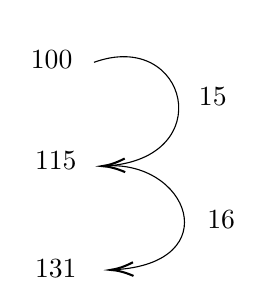
\begin{tikzpicture}[x=0.75pt,y=0.75pt,yscale=-1,xscale=1]
%uncomment if require: \path (0,300); %set diagram left start at 0, and has height of 300

%Curve Lines [id:da8397938007838199] 
\draw    (340.67,91.4) .. controls (385.88,74.97) and (401.36,138.12) .. (346.36,141.32) ;
\draw [shift={(344.67,141.4)}, rotate = 357.99] [color={rgb, 255:red, 0; green, 0; blue, 0 }  ][line width=0.75]    (10.93,-3.29) .. controls (6.95,-1.4) and (3.31,-0.3) .. (0,0) .. controls (3.31,0.3) and (6.95,1.4) .. (10.93,3.29)   ;
%Curve Lines [id:da7421636120725327] 
\draw    (344.67,141.4) .. controls (386.25,137.44) and (405.28,188.37) .. (350.35,191.33) ;
\draw [shift={(348.67,191.4)}, rotate = 357.99] [color={rgb, 255:red, 0; green, 0; blue, 0 }  ][line width=0.75]    (10.93,-3.29) .. controls (6.95,-1.4) and (3.31,-0.3) .. (0,0) .. controls (3.31,0.3) and (6.95,1.4) .. (10.93,3.29)   ;

% Text Node
\draw (309,84.4) node [anchor=north west][inner sep=0.75pt]    {$100$};
% Text Node
\draw (311,133.4) node [anchor=north west][inner sep=0.75pt]    {$115$};
% Text Node
\draw (311,185.4) node [anchor=north west][inner sep=0.75pt]    {$131$};
% Text Node
\draw (390,102.4) node [anchor=north west][inner sep=0.75pt]    {$15$};
% Text Node
\draw (394,161.4) node [anchor=north west][inner sep=0.75pt]    {$16$};


\end{tikzpicture}
\end{center}
\newpage
\begin{quote}
    "Les accidents de la route sont la première cause de mortalité en Belgique"
\end{quote}
Mais cela dépend de comment on définit les causes de mortalité. En effet,
\begin{itemize}
    \item $\left\{\underset{300}{\text{accident}}, \underset{200}{\text{maladies}}, \underset{240}{\text{incendie}}, \underset{200}{\text{naturelle}}, \underset{120}{\text{suicide}}\right\}$
    \item $\left\{\underset{300}{\text{accident}}, \underset{240}{\text{incendie}}, \underset{120}{\text{suicide}}, \underset{400}{\text{naturelle + maladie}}\right\}$
\end{itemize}

\end{remarque}

\underline{\textbf{En dimension 2 : }}

Un échantillons de données se note comme $\{(x_i,y_i)\}_{i=1, \dots , n}$

\begin{enumerate}[label=\arabic*.]
    \item Indicateur univariés : $\bar{x}, \bar{y}, s^2_x, s^2_y, \dots $
    \item Covariance ampirique :
    On pose
    $$
    s_{x,y}= \frac{1}{n}\sum_{i=1}^{n}(x_i-\bar{x})(y_i-\bar{y})= \frac{1}{n} \sum_{i=1}^{n} x_i y_i - \bar{x} \bar{y}
    $$
    On l'interprète de deux manières : 
    \begin{description}
        \item[Interprétation 1 :] Si $s_{x,y} > 0$, un $x_i$ plus grand a tendance à être associé à un $y_i$ plus grand.
        \item[Interprétation 2 :] Si $s_{x,y} < 0$, un $x_i$ plus grand a tendance à être associé à un $y_i$ plus petit.
    \end{description}
    On définit ensuite le coefficient de corrélation :
    $$\operatorname{corr}_{x,y} = \frac{s_{x,y}}{s_x s_y}$$
    \item Nuage de points : 
    Pour un échantillon $\{(x_i,y_i)\}_{i=1,\dots,n}$, on cherche la droite
$\mathcal{D} : y = ax+b$ qui résume la tendance du nuage. Le résidu
d'une observation est l'écart vertical
\[
  \varepsilon_i = y_i - (a x_i + b),
\]
et l'on choisit $(a,b)$ minimisant la somme des carrés des résidus :
\[
  f(a,b) = \sum_{i=1}^{n}\bigl(y_i - (a x_i + b)\bigr)^2
         = \sum_{i=1}^{n}\varepsilon_i^{\,2}.
\]
$f$ étant convexe, le minimum s'obtient en annulant les dérivées
partielles :
\[
  \begin{cases}
    \dfrac{\partial f}{\partial a} = 0\\[2ex]
    \dfrac{\partial f}{\partial b} = 0
  \end{cases}
  \Longrightarrow\quad
  a = \dfrac{s_{xy}}{s_x^{2}},
  \qquad
  b = \bar{y} - \bar{x}\,\dfrac{s_{xy}}{s_x^{2}}.
\]
La pente a donc le signe de $s_{xy}$, et la droite passe par le point
moyen $(\bar{x},\bar{y})$ puisque $y-\bar{y}=a(x-\bar{x})$.
\end{enumerate}

\begin{center}
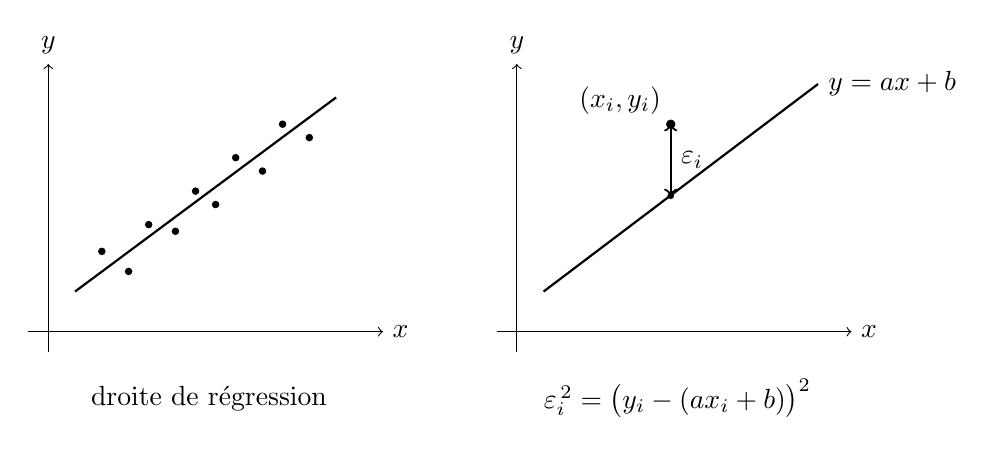
\begin{tikzpicture}[scale=0.85]
  % --- Figure 1 : le nuage ---
  \begin{scope}
    \draw[->] (-0.3,0) -- (5,0) node[right] {$x$};
    \draw[->] (0,-0.3) -- (0,4) node[above] {$y$};
    \draw[thick] (0.4,0.6) -- (4.3,3.5);
    \foreach \p in {(0.8,1.2),(1.2,0.9),(1.5,1.6),(1.9,1.5),
                    (2.2,2.1),(2.5,1.9),(2.8,2.6),(3.2,2.4),
                    (3.5,3.1),(3.9,2.9)}
      \fill \p circle (1.6pt);
    \node at (2.4,-1) {droite de régression};
  \end{scope}

  % --- Figure 2 : le résidu ---
  \begin{scope}[xshift=7cm]
    \draw[->] (-0.3,0) -- (5,0) node[right] {$x$};
    \draw[->] (0,-0.3) -- (0,4) node[above] {$y$};
    \draw[thick] (0.4,0.6) -- (4.5,3.7)
      node[right] {$y=ax+b$};
    \coordinate (P) at (2.3,3.1);
    \coordinate (Q) at (2.3,2.03);
    \fill (P) circle (2pt) node[above left] {$(x_i,y_i)$};
    \fill (Q) circle (1.4pt);
    \draw[<->, thick] (P) -- (Q) node[midway,right] {$\varepsilon_i$};
    \node at (2.4,-1) {$\varepsilon_i^{\,2}=\bigl(y_i-(ax_i+b)\bigr)^2$};
  \end{scope}
\end{tikzpicture}
\end{center}




